\subsection{De Turingmachine als herkenner en beslisser}

\vspace{0.5cm}

\begin{theo}[Turingmachine]{Turingmachine}
    Een \textbf{Turingmachine} is een 7-tal $(Q, \Sigma, \Gamma, \delta, q_0, q_{a}, q_{r})$ waarbij $Q, \Sigma, \Gamma$ eindige verzamelingen zijn en 
    
    \vspace{0.3cm}\begin{minipage}{0.56\textwidth}
        \begin{itemize}
            \item $Q$ is een verzameling toestanden
            \item $\Sigma$ is het input alfabet dat $\#$ niet bevat
            \item $\Gamma$ is het tape alfabet waarbij $\Sigma \subset \Gamma$ en $\# \in \Gamma$
            \item $q_s$ is de starttoestand
            \item $q_a$ is de accepterende eindtoestand
            \item $q_r$ is de verwerpende eindtoestand, verschillend van $q_a$
            \item $\delta$ is de transitiefunctie: een totale functie met signatuur
            \begin{equation*}
                Q \times \Gamma \rightarrow Q \times \Gamma \times \{L, R, S\}
            \end{equation*}
        \end{itemize}
    \end{minipage}
    \hspace{0.2cm}\begin{minipage}{0.4\textwidth}
        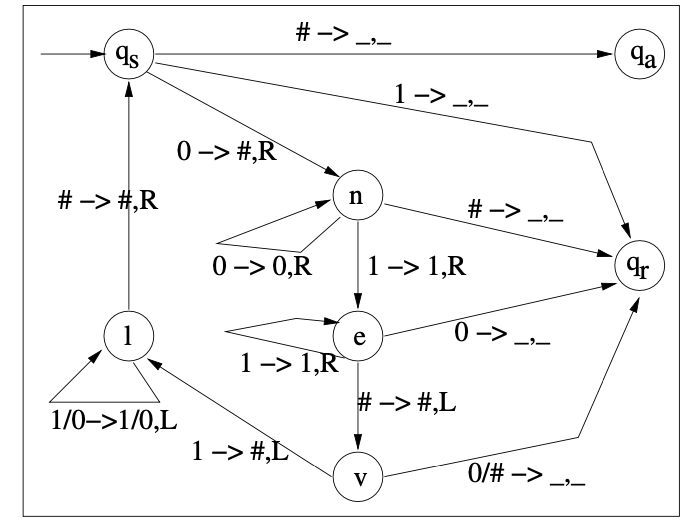
\includegraphics[scale = 0.27]{Images/TuringmachineEx.png}
    \end{minipage}
\end{theo}

% \begin{theo}[Herkennen]{Herkennen}
%     Een Turingmachine TM \textbf{herkent} een taal $L$
% \end{theo}

\begin{theo}[Turing-herkenbare taal]{Turing-herkenbare taal}
    Een taal L is \textbf{Turing-herkenbaar} als er een Turingmachine TM bestaat zodanig dat
    \begin{equation*}
        L = L_{\text{TM}}.
    \end{equation*}
    \textbf{Opmerking:} $\infty_{\text{TM}}$ is niet leeg: voor elke string niet in $L$ gaat de machine in een lus.
\end{theo}

\begin{theo}[Turing-beslisbare taal]{Turing-beslisbare taal}
    Een taal L is \textbf{Turing-beslisbaar} als er een Turingmachine TM bestaat zodanig dat
    \begin{equation*}
        L = L_{\text{TM}} \text{ en } \infty_{\text{TM}} = \emptyset.
    \end{equation*}
    \vspace{-0.3cm}
\end{theo}

\begin{theo}[Co-herkenbaar/co-beslisbaar]{Co-herkenbaar/co-beslisbaar}
    Een taal $L$ is co-herkenbaar/co-beslisbaar als $\overline{L}$ herkenbaar/beslisbaar is.
\end{theo}

\newpage

\begin{lem}[Turing-beslisbaarheid en Turing-herkenbaarheid]{Turing-beslisbaarheid en Turing-herkenbaarheid}
    \begin{enumerate}
        \item Als een taal $L$ beslisbaar is, dan is $L$ co-beslisbaar.
        \item Als een taal $L$ herkenbaar en co-herkenbaar is, dan is $L$ beslisbaar.
        \item Er bestaat een taal die niet herkenbaar is.
    \end{enumerate}
\end{lem}

\begin{prf}[Turing-beslisbaarheid en Turing-herkenbaarheid]{Turing-beslisbaarheid en Turing-herkenbaarheid}
    \begin{enumerate}
        \item 
            Verwissel de rol van $q_a$ en $q_r$ in de Turingmachine die $L$ beslist.
        \item 
            Laat $M_1$ de machine zijn die $L$ herkent, en $M_2$ de machine die $\overline{L}$ herkent. De idee is nu dat we $M_1$ en $M_2$ samen laten lopen als een nieuwe machine $M$, in parallel: zodra $M_1$ accepteert, dan accepteert $M$, en zodra $M_2$ accepteert, dan verwerpt $M$. $M_1$ en $M_2$ kunnen niet samen accepteren, en voor elke string zal minstens één van de machines $M_1$ en $M_2$ stoppen p in zijn aanvaardende toestand. $M$ beslist $L$.
        \item 
            Het bewijs steunt op het begrip kardinaliteit: we weten van vroeger dat het aantal Turingmachines aftelbaar oneindig is. We weten ook dat elke Turingmachine juist één taal herkent. En tenslotte weten we ook dat het aantal talen niet-aftelbaar oneindig is, want de verzameling talen is $\mathcal{P}(\Sigma^*)$. Bijgevolg bestaat een niet-herkenbare taal. In feite is daarmee zelfs bewezen dat er niet-aftelbaar veel niet-herkenbare talen bestaan. Meer nog: bijna alle talen zijn niet-herkenbaar!
    \end{enumerate}
\end{prf}

\subsection{Encodering}

\vspace{0.5cm}

\begin{theo}[Encodering]{Encodering}
    Een encodering is een mapping van objecten in $\Sigma$ naar strings in $\Sigma^*$. Encoderingen zijn \textbf{redelijk}:
    \begin{itemize}
        \item Elk object moet minstens 1 encodering in $\Sigma^*$ hebben.
        \item Elke encodering moet volledig het object dat het encodeert bepalen.
        \item De nodige operaties moeten berekenbaar zijn uit de encodering van de objecten.
        \item Een redelijke encodering introduceert geen extra informatie.
    \end{itemize}
\end{theo}

\begin{theo}[Universele Turingmachine]{Universele Turingmachine}
    De Universele Turingmachine kan elke TM simuleren, als die maar geëncodeerd wordt zoals nodig: we kunnen de UTM zelfs laten beginnen met controleren of wat op de banden staat wel een geldige encodering is.
\end{theo}

\subsection{Het Halting-probleem}

\vspace{0.5cm}

\begin{theo}[Acceptatieprobleem]{Acceptatieprobleem}
    Stel een Turingmachine M voor met een input $w$. De \textbf{acceptatietaal} A$_{\text{TM}}$ is 
    \begin{equation*}
        \text{A}_{\text{TM}} = \{ \langle M,s \rangle \ | \ M \text{ is een Turingmachine en } s \in L_{\text{M}} \}
    \end{equation*}
    zodanig dat de Turingmachine A de taal \textbf{beslist}. Dit is een verwant probleem aan het Halting-probleem.
    \vspace{-0.5cm}
\end{theo}

\begin{lem}[Acceptatietaal is niet beslisbaar, maar wel herkenbaar]{Acceptatietaal is niet beslisbaar, maar wel herkenbaar}
    A$_{\text{TM}}$ is niet beslisbaar, maar A$_{\text{TM}}$ is herkenbaar.
\end{lem}

\begin{prf}[Acceptatietaal is niet beslisbaar, maar wel herkenbaar]{prf - Acceptatietaal is niet beslisbaar, maar wel herkenbaar}
    \begin{itemize}
        \item 
            We bewijzen door middel van contradictie. Stel er bestaat een beslisser B voor A$_{\text{TM}}$. Dat betekent dat bij input $\langle \text{M},s \rangle$ B accepteert als M bij input $s$ stopt in $q_a$ en verwerpt als M bij input $s$ niet accepteert, dus stopt in zijn $q_r$ of loopt. We schrijven
            \begin{equation*}
                \text{B}(\langle \text{M},s \rangle) \ \text{is accept als M} \ s \ \text{accepteert en anders reject}.
            \end{equation*}
            Gebruikmakend van B kunnen we nu de contradictie machine C construeren, Deze neemt als input (de codering van) een Turingmachine M, roept B op met input $\langle \text{M}, \text{M} \rangle$, en als B accepteert dan verwerpt C en omgekeerd. Kortom, C heeft de eigenschap:
            \begin{equation*}
                \forall M \in \text{Turingmachines}: \ \text{C}(\langle \text{M} \rangle) = \text{opposite}(\text{B}(\langle \text{M}, \text{M} \rangle)).
            \end{equation*}
            Neem nu voor M hierboven C zelf, dan krijgen we:
            \begin{equation*}
                \hspace{2cm}\text{C}(\langle \text{C} \rangle) = \text{opposite}(\text{B}(\langle \text{C}, \text{C} \rangle)).
            \end{equation*}
            Er geldt nu het volgende:
            \begin{align*}
                \hspace{2cm}
                C \ \text{accepteert} \ C 
                    &\Leftrightarrow C(\langle C \rangle) = \text{accept} \\
                    &\Leftrightarrow \text{opposite}(\text{B}(\langle C, C \rangle)) = \text{reject} \\
                    &\Leftrightarrow C \ \text{verwerpt} \ C.
            \end{align*}
            Dit is een contradictie, dus B kan niet bestaan en is $A_{\text{TM}}$ niet beslisbaar.
        \item 
            De herkenner H voor A$_{\text{TM}}$ laat gewooon bij input $\langle \text{M},s \rangle$ de machine M lopen op input s: als M accepteert, dan accepteert H. Als M verwerpt of loopt, dan loopt H ook.
    \end{itemize}
    \vspace{-0.3cm}
\end{prf}

\newpage

\begin{theo}[Halting-probleem]{Halting-probleme}
    Stel een Turingmachine M voor met een input $w$. De \textbf{haltingtaal} H$_{\text{TM}}$ is 
    \begin{equation*}
        \text{H}_{\text{TM}} = \{ \langle M,s \rangle \ | \ M \text{ is een Turingmachine die stopt bij input } s \}
    \end{equation*}
    zodanig dat de Turingmachine H de taal \textbf{beslist}.
\end{theo} 

\begin{lem}[Halting-taal is niet beslisbaar, maar wel herkenbaar]{Halting-taal is niet beslisbaar, maar wel herkenbaar}
    H$_{\text{TM}}$ is niet beslisbaar, maar H$_{\text{TM}}$ is herkenbaar.
\end{lem}

\begin{prf}[Halting-taal is niet beslisbaar, maar wel herkenbaar]{prf - Halting-taal is niet beslisbaar, maar wel herkenbaar}
    \begin{itemize}
        \item 
            Stel dat H$_{\text{HM}}$ beslisbaar is door een Turingmachine H. We construeren nu beslisser B voor A$_{\text{HM}}$ als volgt: bij input $\langle \text{M} ,s \rangle$ doet B:
            \begin{itemize}
                \item laat eerst H lopen op $\langle \text{M} ,s \rangle$
                \item $H(\langle \text{M} ,s \rangle) = \text{accept} \Rightarrow$ B accepteert en geeft als resultaat wat M geeft 
                \item $H(\langle \text{M} ,s \rangle) = \text{reject} \Rightarrow$ reject B ook de string $\langle \text{M} ,s \rangle$. 
            \end{itemize}
            Vermits er geen beslisser voor A$_{\text{HM}}$ bestaat, kan H niet bestaan en is dus ook H$_{\text{HM}}$ niet beslisbaar zijn.
        \item
            De herkenner H voor H$_{\text{HM}}$ laat gewoon bij input $\langle \text{M} ,s \rangle$ de machine M lopen op input s: als M stopt, dan accepteert H. Als M loopt, dan loopt H ook.
    \end{itemize}
\end{prf}

\begin{lem}[De complemententalen zijn niet herkanbaar]{De complemententalen zijn niet herkanbaar}
    $\overline{\text{A}_{\text{TM}}}$ en $\overline{\text{H}_{\text{TM}}}$ zijn niet herkenbaar.
\end{lem}

\begin{prf}[De complemententalen zijn niet herkanbaar]{prf - De complemententalen zijn niet herkanbaar}
    \begin{itemize}
        \item 
            Als $\overline{\text{A}_{\text{TM}}}$ herkenbaar is,en vermits herkenbaar is, dan is ook $\text{A}_{\text{TM}}$ beslisbaar. Maar dat is niet het geval, dus $\overline{\text{A}_{\text{TM}}}$ is niet herkenbaar.
        \item 
            Als $\overline{\text{H}_{\text{TM}}}$ herkenbaar is,en vermits herkenbaar is, dan is ook $\text{H}_{\text{TM}}$ beslisbaar. Maar dat is niet het geval, dus $\overline{\text{H}_{\text{TM}}}$ is niet herkenbaar.
    \end{itemize}
\end{prf}

\newpage

\subsection{De enumeratormachine}

\vspace{0.5cm}

\begin{lem}[Enumeratormachine]{Enumeratormachine}
    De taal door een enumerator bepaald is herkenbaar en elke herkenbare taal wordt door een enumerator geënumereerd.
\end{lem}

\begin{prf}[Enumeratormachine]{prf - Enumeratormachine}
    \begin{itemize}
        \item 
            We beschrijven informeel een herkenner TM voor de taal $L$ bepaald door een gegeven enumerator Enu: TM gebruikt Enu als subruitine als volgt. Geef een string $s$ aan de TM\@. De TM start de Enu. Telkens de Enu in zijn $q_e$ komt, kijkt TM na of de laatst geproduceerde string op de outputband van de Enu gelijk is aan $s$. Indien ja: TM accepteert. Indien niet, laat de Enu verderrekenen.
        \item 
            Laat de TM $L$ bepalen. We construeren de Enu voor die $L$ als volgt. Maak eerst een TM$_{\text{gen}}$ die bij input een getal $n$, het getal $n$ gevolgd door de eerste $n$ strings uit $\Sigma^*$ op de band zet: $n, s_1, s_2, \dots, s_n$. Maak een TM die bij input $n, s_1, s_2, \dots, s_n$ $n$ stappen van TM uitvoert op elk van de $n$ strings: als daarbij een string $s_i$ geaccepteerd wordt, schrijf die dan op de outputband voor Enu. Maak nu een TM$_{\text{driver}}$ die de opeenvolgende getallen $n$ genereert en dan TM$_{\text{gen}}$ en TM oproept.
            Waarom is dit algoritme correct? Als TM een string $s$ aanvaardt, bv\@. in $m$ stappen, zal Enu $s$ op de output zetten tijdens iteratie $n$ bij voldoende grote $n$, namelijk, zodat $s$ valt binnen $s_1,\ldots,s_n$ en zodat $n \geq m$. Merk op dat Enu $s$ oneindig vaak op de output band zal zetten.
    \end{itemize}
\end{prf}

\newpage

\subsection{Beslisbare talen}

\vspace{0.3cm}

\begin{lem}[Encoderingen van reguliere talen zijn beslisbaar]{Encoderingen van reguliere talen zijn beslisbaar}
    \vspace{-0.1cm}
    De talen
    \begin{itemize}
        \item 
            A$_{\text{DFA}} = \{\langle \text{D}, s\rangle\  | \ \text{D is een DFA en D accepteert $s$} \}$
        \item 
            A$_{\text{NFA}} = \{\langle \text{N}, s\rangle\  | \ \text{N is een NFA en D accepteert $s$} \}$
        \item 
            A$_{\text{RegExp}} = \{\langle \text{R}, s\rangle\  | \ \text{R is een reguliere expressie en R genereert $s$} \}$
    \end{itemize}
    zijn beslisbaar.
    \vspace{-0.1cm}
\end{lem}

\begin{prf}[Beslisbare talen]{prf - Beslisbare talen}
    \vspace{-0.1cm}
    \begin{itemize}
        \item 
            De beslisser B krijgt als input $\langle \text{D}, s\rangle$. B simuleert D op $s$. Als D $s$ accepteert, dan stopt B in zijn $q_a$ en accepteert. Als D $s$ verwerpt, dan stopt B in zijn $q_r$ en verwerpt. Er is geen probleem met niet stoppen.
        \item 
            De beslisser B krijgt als input $\langle \text{N}, s\rangle$. B zet N om in een DFA D en roept de beslisser voor A$_{\text{DFA}}$ op met input $\langle \text{D}, s\rangle$.
        \item 
            De beslisser B krijgt als input $\langle \text{R}, s\rangle$. B zet R om in een NFA N en roept de beslisser voor A$_{\text{NFA}}$ op met input $\langle \text{N}, s\rangle$.
    \end{itemize}
    \vspace{-0.3cm}
\end{prf}

\begin{lem}[Encoderingen van reguliere talen zijn beslisbaar - gevolg]{Encoderingen van reguliere talen zijn beslisbaar - gevolg}
    \vspace{-0.1cm}
    De talen
    \begin{itemize}
        \item 
            $\mathcal{E}_{\text{DFA}} = \{\langle \text{DFA} \rangle \ | \ \text{$\epsilon \in$ L$_{\text{DFA}}$} \}$
        \item 
            $\text{E}_{\text{DFA}} = \{\langle \text{DFA} \rangle \ | \ \text{L$_{\text{DFA}}$ = $\phi$} \}$
        \item 
            $\text{EQ}_{\text{DFA}} = \{\langle \text{DFA$_1$}, \text{DFA$_2$} \rangle \ | \ \text{L$_{\text{DFA$_1$}}$ = L$_{\text{DFA$_2$}}$} \}$
    \end{itemize}
    zijn beslisbaar.
    \vspace{-0.1cm}
\end{lem}

\begin{prf}[Encoderingen van reguliere talen zijn beslisbaar - gevolg]{prf - Encoderingen van reguliere talen zijn beslisbaar - gevolg}
    \begin{itemize}
        \item 
            Dit bewijs is triviaal, want A$_{\text{DFA}}$ is beslisbaar.
        \item 
            Stel B een beslisser voor $\text{E}_{\text{DFA}}$. B krijgt als input (een codering van) de DFA\@. B checkt of dat een eindtoestand bereikbaar is vanuit de starttoestand. Indien ja, dan verwerpt B. Indien nee, dan accepteert B.
        \item 
            Uit DFA$_1$ en DFA$_2$ construeer je de DFA$_{\Delta}$ die het symmetrisch verschil tussen L$_{\text{DFA}_1}$ en L$_{\text{DFA}_2}$ bepaalt. Beslis dan of DFA$_{\Delta}$ de lege taal bepaalt, zie bewijs hierboven.
    \end{itemize}
\end{prf}

\begin{lem}[Encodering van een contextvrije taal is beslisbaar]{Encodering van een contextvrije taal is beslisbaar}
    Aanvaarden van een string door een CFG
    \begin{equation*}
        \text{A}_{\text{CFG}} = \{\langle \text{G}, s\rangle\  | \ \text{G is een CFG en $s \in L_{\text{G}}$} \}
    \end{equation*}
    is beslisbaar.
\end{lem}

\begin{prf}[Encodering van een contextvrije taal is beslisbaar]{prf - Encodering van een contextvrije taal is beslisbaar}
    Stel B een beslisser voor $\text{A}_{\text{CFG}}$. Bij input $\langle \text{G}, s\rangle$, converteer G eerst naar zijn Chomsky Normaal Vorm. Geneer alle mogelijke strings met een derivatielengte $2|s| - 1$: dat zijn er eindig veel. B controleert of $s$ daarbij zit. Indien ja, dan accepteert B. Indien nee, dan verwerpt B.
\end{prf}

\begin{lem}[Encodering van een contextvrije taal is beslisbaar - gevolg]{prf - Encodering van een contextvrije taal is beslisbaar - gevolg}
    De talen
    \begin{itemize}
        \item 
            $ \text{E}_{\text{CFG}} = \{\langle \text{G} \rangle\  | \ \text{G is een CFG en $L_{\text{G}} = \phi$} \}$
        \item 
            $ \text{ES}_{\text{CFG}} = \{\langle \text{G} \rangle\  | \ \text{G is een CFG en $\epsilon \in L_{\text{G}}$} \}$
    \end{itemize}
    zijn beslisbaar.
\end{lem}

\begin{prf}[Leegheid van een CFG is beslisbaar]{prf - Leegheid van een CFG is beslisbaar}
    \begin{itemize}
        \item 
            We beschrijven informeel een algoritme dat G transformeert naar een vorm waarin de beslissing gemakkelijk is.
            \begin{itemize}
                \item 
                    als er een regel $A \to \alpha$ in zit, en $\alpha$ bestaat alleen uit eindsymbolen (mag dus ook $\epsilon$ zijn), dan 
                    \begin{itemize}
                        \item verwijder alle regels waar A aan de linkerkant staat
                        \item vervang in elke regel waar A rechts voorkomt, de voorkomens van A door $\alpha$
                    \end{itemize}
                \item 
                    blijf dit doen totdat ofwel
                    \begin{itemize}
                        \item het startsymbool verwijderd is: reject, want het startsymbool kan een string afleiden
                        \item er geen regels zijn van de benodigde vorm: accept, want de taal is leeg
                    \end{itemize}
            \end{itemize}
            Het algoritme is eindig, omdat elke iteratie minstens één regel verwijdert en er een eindig aantal regels zijn. Het algoritme is correct, want als de taal leeg is, dan zal het algoritme dat ook vinden. Als de taal niet leeg is, dan zal het algoritme dat ook vinden.
        \item 
            We transformeren de CFG naar zijn Chomsky Normaal Vorm. Indien die de regel $S \to \epsilon$ bevat, dan accepteren we. Indien niet, dan verwerpen we.
    \end{itemize}
\end{prf}

\begin{lem}[Beslisbaarheid van CFL]{Beslisbaarheid van CFL}
    Elke contextvrije taal is beslisbaar.
\end{lem}

\begin{prf}[Beslisbaarheid van CFL]{prf - Beslisbaarheid van CFL}
    We zouden voor de CFL $L$ een PDA kunnen kiezen die $L$ beslist en deze PDA omzetten in een Turingmachine. Het probleem is dat een PDA in het algemeen niet-deterministisch is, en dus direct overeenkomt met een niet-deterministische TM\@. Maar zo'n NTM kan omgezet worden tot een TM die $L$ beslist. Een alternatief is om een CFG G voor $L$ te nemen en aan te tonen dat een beslisser B$_\text{G}$ bestaat die voor elke string $s$ kan beslissen of die door G wordt gegenereerd. Dat is natuurlijk niet hetzelfde als A$_{\text{CFG}}$ beslissen, maar het terkt er wel op. We kunnen B$_\text{G}$ als volgt construeren: we zetten G eerst om in zijn Chomsky Normaal Vorm. We genereren dan alle strings met een derivatielengte $2|s| - 1$: dat zijn er eindig veel. B$_\text{G}$ controleert of $s$ daarbij zit. Indien ja, dan accepteert B$_\text{G}$. Indien nee, dan verwerpt B$_\text{G}$.
\end{prf}

\subsection{Niet-beslisbare talen}

\vspace{0.5cm}

\begin{lem}[Niet-beslisbare talen]{Niet-beslisbare talen}
    De talen
    \begin{itemize}
        \item 
            $\text{E}_{\text{TM}} = \{\langle \text{M} \rangle \ | \ \text{M is een TM en} \ \text{L$_{\text{M}}$ = $\phi$} \}$
        \item 
            $\text{REGULAR}_{\text{TM}}$
        \item 
            $\text{EQ}_{\text{TM}}$
    \end{itemize}
    zijn niet-beslisbaar.
\end{lem}

\begin{prf}[Niet-beslisbare talen]{prf - Niet-beslisbare talen}
    \begin{itemize}
        \item 
            Het idee van het bewijs is om aan te tonen dat we met een code $\langle \text{M}, s \rangle$, een Turingmachine $\text{M}_{\langle \text{M}, s \rangle}$ kunnen berekenen zodat 
            \begin{equation*}
                \langle \text{M}, s \rangle \in \text{A}_{\text{TM}} 
                \ \Leftrightarrow \
                \text{M}_{\langle \text{M}, s \rangle} \in \text{E}_{\text{TM}}.
            \end{equation*}
            $\text{M}_{\langle \text{M}, s \rangle}$ doet het volgende met input $w$: het test of $w \neq s$; zo ja dan volgt een reject; zo niet wordt M op $w$ gesimuleerd. Als M eindigt wordt het resultaat van M teruggeven. Het is duidelijk dat bij input $\langle \text{M}, s \rangle$, $\text{M}_{\langle \text{M}, s \rangle}$ berekend kan worden. Verder geldt dat $L_{\text{M}_{\langle \text{M}, s \rangle}} = \emptyset$ indien $\langle \text{M}, s \rangle \notin \text{A}_{\text{TM}}$ en $L_{\text{M}_{\langle \text{M}, s \rangle}} = \{s\}$ indien $\langle \text{M}, s \rangle \in \text{A}_{\text{TM}}$.  Bijgevolg,
            \begin{equation*}
                \langle \text{M}, s \rangle \notin \text{A}_{\text{TM}}
                \ \Leftrightarrow \
                \langle \text{M}_{\langle \text{M}, s \rangle} \rangle \in \text{E}_{\text{TM}}.
            \end{equation*}
            Stel dat $\text{E}_{\text{TM}}$ een beslisser E bezit. Construeer nu een beslisser B voor $\text{A}_{\text{TM}}$ als volgt: bij input $\langle \text{M}, s \rangle$, berekent B de code $\langle \text{M}_{\langle \text{M}, s \rangle} \rangle$ van $\text{M}_{\langle \text{M}, s \rangle}$ en voert E uit op deze code. Indien E reject, dan eindigt B met accept; indien E accepteert, dan eindigt B met reject. Sinds een beslisser B voor $\text{A}_{\text{TM}}$ niet bestaat, kan $\text{E}_{\text{TM}}$ niet beslisbaar zijn.
        \item 
            We laten zien dat we voor elk paar $\langle \text{M}, s \rangle$ een TM $\text{M}_{\langle \text{M}, s \rangle}$ kunnen berekenen met de eigenschap dat $\text{L}_{\text{M}_{\langle \text{M}, s \rangle}}$ gelijk is aan de reguliere taal $\Sigma^*$ indien M $s$ accepteert, en gelijk is aan de niet-reguliere taal $\{ 0^n1^n \ | \ n \in \mathbb{N} \}$ indien M $s$ niet accepteert. Op deze $\langle \text{M}, s \rangle$ junnen we vervolgens een beslisser voor $\text{REGULAR}_{\text{TM}}$ toepassen om te beslissen of M $s$ accepteert. Dit leidt tot contradictie. Voor elk paar $\langle \text{M}, s \rangle$ doet $\text{M}_{\langle \text{M}, s \rangle}$ het volgende bij input w: het berekent of w van de vorm $0^n1^n$ is (gebruikmakend van de beslisser). Zo ja, dan stopt $\text{M}_{\langle \text{M}, s \rangle}$ met accept; zo niet, dan wordt M gesimuleerd op $s$; indien M eindigt, dan eindigt $\text{M}_{\langle \text{M}, s \rangle}$ in dezelfde eindtoestand als M. Stel dat $\text{REGULAR}_{\text{TM}}$ een beslisser R bezit. Construeer nu een beslisser B voor A$_{\text{TM}}$ als volgt: bij input $\langle \text{M}, s \rangle$, berekent B de code $\langle \text{M}_{\langle \text{M}, s \rangle} \rangle$ van $\text{M}_{\langle \text{M}, s \rangle}$ en voert R uit op deze code. Indien R accepteert, dan is $\text{L}_{\text{M}_{\langle \text{M}, s \rangle}} = \Sigma^*$, en dan eindigt B met accept; indien E reject, dan is $\text{L}_{\text{M}_{\langle \text{M}, s \rangle}} = \{ 0^n1^n \ | \ n \in \mathbb{N} \}$, en dan eindigt B met reject. Sinds een beslisser B voor $\text{A}_{\text{TM}}$ niet bestaat, kan $\text{REGULAR}_{\text{TM}}$ niet beslisbaar zijn.
        \item 
            We weten al dat $\text{E}_{\text{TM}}$ niet beslisbaar is, en eigenlijk kan dat probleem beschouwd worden als een speciaal geval van het equivalentieprobleem: namelijk het probleem om te beslissen of een TM equivalent is met M$_{\phi}$. Dus, als $\text{EQ}_{\text{TM}}$ beslisbaar is, dan is $\text{E}_{\text{TM}}$ ook beslisbaar, wat een contradictie is.
    \end{itemize}
\end{prf}

\begin{theo}[Lineair Begrensde Automaat]{Lineair Begrensde Automaat}
    Een Lineair Begrensde Automaat is een Turingmachine die niet leest of schrijft buiten het deel van de band dat initieel invoer bevat.
\end{theo}

\begin{lem}[Acceptatieprobleem bij LBA]{Acceptatieprobleem bij LBA}
    $\text{A}_{\text{LBA}}$ is beslisbaar.
\end{lem}

\begin{prf}[Acceptatieprobleem bij LBA]{prf - Acceptatieprobleem bij LBA}
    We kijken naar de configuraties die kunnen voorkomen tijdens de uitvoering van een LBA op een string met lengte $n$. Het aantal toestanden van de LBA noteren we met $q$ en het aantal elementen in het bandalfabet met $b$. Het aantal mogelijke strings die tijdens de uitvoering op de band kunnen staan is begrensd door $b^n$. De leeskop kan onder elk van de symbolen staan terwijl de machine in elk van de toestanden kan zitten. Dat geeft in het totaal maximaal $qnb^n$ configuraties. We kunnen nu een beslisser B voor $\text{A}_{\text{LBA}}$ construeren als volgt: bij input $\langle \text{M}, s \rangle$ doet B het volgende 
    \begin{itemize}
        \item berekent $\text{M}ax = qnb^n$,
        \item simuleert dan M op $s$ voor maximaal $\text{M}ax$ stappen, \item indien M ondertussen accepteerde, accept; indien M ondertussen verwierp, reject,
        \item indien M ondertussen niet stopte, reject.
    \end{itemize}
    B is een beslisser, omdat M op $s$ stopt na maximaal $\text{M}ax$ stappen en sinds een beslisser B voor $\text{A}_{\text{LBA}}$ bestaat, is $\text{A}_{\text{LBA}}$ beslisbaar.
\end{prf}

\begin{lem}[Leegheid van een LBA]{Leegheid van een LBA}
    De taal 
    \begin{equation*}
        \text{E}_{\text{LBA}} = \{\langle \text{M} \rangle \ | \ \text{M is een LBA en} \ \text{L$_{\text{M}}$ = $\phi$} \}
    \end{equation*}
    is niet beslisbaar.
\end{lem}

\begin{prf}[Leegheid van een LBA]{prf - Leegheid van een LBA}
    Stel dat E een beslisser voor $\text{E}_{\text{LBA}}$ is. We construeren nu een beslisser B voor $\text{A}_{\text{TM}}$ als volgt: bij input $\langle \text{M}, s \rangle$ doet B het volgende
    \begin{itemize}
        \item construeert de LBA $\text{A}_{\text{M},s}$ die voor een input $x$ kan beslissen of $x$ een accepterende computation history
        \begin{equation*}
            C \in \Gamma^*Q\Gamma^*: \ \#C_0\#\ldots\#C_n\#
        \end{equation*}
        is van M voor input $s$;
        \item laat E los op $\langle \text{A}_{\text{M},s} \rangle$: als E aanvaardt, reject; anders accept;
    \end{itemize}
    B beslist $\text{A}_{\text{TM}}$, want
    \begin{align*}
        \hspace{4cm}
        \text{B accepteert} \ \langle \text{M}, s \rangle  
        &\Leftrightarrow \text{E rejects} \ \langle \text{A}_{\text{M},s} \rangle \\ 
        &\Leftrightarrow \text{A}_{\text{M},s} \ \text{aanvaardt minstens één string} \\
        &\Leftrightarrow \text{er bestaat een computation history van M voor $s$} 
    \end{align*}
    Het laatste is equivalent met zeggen dat M de string $s$ accepteert. Dus is B een beslisser van $\text{A}_{\text{TM}}$, wat tot een contradictie leidt. Dus E bestaat niet en is $\text{E}_{\text{LBA}}$ niet beslisbaar.
\end{prf}

\subsection{De stelling van Rice}

\vspace{0.5cm}

\begin{theo}[Niet-triviale eigenschap]{Niet-triviale eigenschap}
    Een eigenschap $P$ van Turingmachines heet \textbf{niet-triviaal} indien 
    \begin{equation*}
        P \neq \emptyset \ \land \ P^c \neq \emptyset. 
    \end{equation*}
    \vspace{-0.5cm}
\end{theo}

\begin{theo}[Taal-invariante eigenschap]{Taal-invariante eigenschap}
    De eigenschap $P$ van Turingmachines is \textbf{taal-invariant} indien 
    \begin{equation*}
        \text{L}_{\text{M}_1} = \text{L}_{\text{M}_2}
        \Rightarrow
        P(\text{M}_1) = P(\text{M}_2).
    \end{equation*}
    of in woorden alle machines die dezelfde taal bepalen hebben ofwel allemaal $P$, ofwel heeft geen enkele ervan $P$.
\end{theo}

\begin{lem}[Stelling I van Rice]{Stelling van Rice}
    Voor elke niet-triviale, taal-invariante eigenschap $P$ van Turingmachines is de taal 
    \begin{equation*}
        \text{POS}_P = \{\langle \text{M} \rangle \ | \ \text{M} \in P\}
    \end{equation*}
    niet beslisbaar.
\end{lem}

\begin{prf}[Stelling I van Rice]{prf - Stelling van Rice}
    Eerst tonnen we aan dat voor elke input $\langle \text{M}, s \rangle$ voor $\text{A}_{\text{TM}}$ een TM $\text{M}_{\langle \text{M}, s \rangle}$ kan berekend worden zodat
    \begin{equation*}
        \langle \text{M}, s \rangle \in \text{A}_{\text{TM}} 
        \ \Leftrightarrow \
        \langle \text{M}_{\langle \text{M}, s \rangle} \rangle \in \text{POS}_P.
    \end{equation*}
    Kies twee TM's, M$_{\emptyset}$ en een TM X zodat 
    \begin{equation*}
        P(\text{X}) \neq P(\text{M}_{\emptyset}).
    \end{equation*}
    Aangezien $P$ niet triviaal is, bestaat er zo'n X. We veronderstellen eerst dat M$_{\emptyset}$ niet voldoet aan $P$; dan voldoet X wel aan $P$. (Als M$_{\emptyset}$ wel voldoet aan $P$, verwissel dan $P$ en $\overline{P}$. Uit de rest van het bewijs volgt dan dat POS$_{\overline{P}}$ onbeslisbaar is, dus ook POS$_P$.) Voor input $\langle \text{M}, s \rangle$ voor A$_{\text{TM}}$ kan de volgende TM M$_{\langle \text{M}, s \rangle}$ berekend worden: bij input w wordt eerst M gesimuleerd op $s$; als M rejects, dan zal M$_{\langle \text{M}, s \rangle}$ rejecten; als M accepteert, dan wordt X gesimuleerd op $w$l als X eindigt, dan stopt M$_{\langle \text{M}, s \rangle}$ in dezelfde eindtoestand als X. We stellen vast dat de taal L$_{\text{M}_{\langle \text{M}, s \rangle}}$ geaccepteerd door M$_{\langle \text{M}, s \rangle}$ gelijk is aan $\emptyset$ indien M $s$ niet accepteert en gelijk is aan L$_{\text{X}}$ indien M $s$ wel accepteert. Uit de taal-invariantie van $P$ volgt 
    \begin{equation*}
        \text{M}_{\langle \text{M}, s \rangle} \ \text{heeft de eigenschap} \ P
        \ \Leftrightarrow \ 
        \text{M} \ \text{accepteert} \ s.
    \end{equation*}
    Stel dat POS$_P$ een beslisser E heeft. Construeer nu een TM B die bij input $\langle \text{M}, s \rangle$, de code $\langle \text{M}_{\langle \text{M}, s \rangle} \rangle$ berekent en hierop E uitvoert. Dan is B een beslisser voor A$_{\text{TM}}$, wat een contradictie is. Dus E bestaat niet en is POS$_P$ niet beslisbaar.
\end{prf}

\subsection{Het Post Correspondence Problem}

\vspace{0.5cm}

\begin{lem}[Toepassing van PCP's]{Toepassing van PCP's}
    De taal 
    \begin{equation*}
        \{ < \text{M}, \text{N} > \ | \ \text{M,N zijn PDA's en} \ \text{L}_{\text{M}} \cap \text{L}_{\text{n}} \neq \emptyset \}
    \end{equation*}
    is niet beslisbaar.
\end{lem}

\newpage

\begin{prf}[Toepassing van PCP's]{prf -Toepassing van PCP's}
    We kunnen dit aantonen door een reductie te maken van het beslissen van een Post Correspondence Probleem, naar bovenstaande taal. Een PCP bestaat uit $k$ stenen: $a_1/b_1, \ldots, a_k/b_k$. We kunnen een dergelijke PCP omzetten in 2 PDA's. De eerste is de PDA die de volgende CFG implementeert
    \begin{align*}
        S &\to a_1 A t_1 \ | \ \ldots \ | \ a_k A t_k \\
        A &\to \epsilon \ | \ S,
    \end{align*}
    de tweede is de PDA die de volgende CFG implementeert
    \begin{align*}
        S &\to b_1 B t_1 \ | \ \ldots \ | \ b_k B t_k \\
        B &\to \epsilon \ | \ S
    \end{align*}
    waarbij $t_1, \ldots, t_k$ nieuwe symbolen zijn die elk uniek een steen identificeren. De strings van de eerste taal bestaan uit strings samengesteld uit de $a_i$'s bovenop de stenen van het spel, gevolgd door de omgekeerde rij van symbolen $t_i$ die aangeeft welke stenen gebruikt zijn. Analoog bestaan de strings van de tweede taal uit strings die gevormd kunnen worden met strings $b_i$ onderaan op de stenen, gevolgd door de omgekeerde rij van symbolen $t_i$ van de gebruikte stenen. Een string in de doorsnede van deze twee talen geeft een sequentie van stenen zodat de string bovenaan en onderaan identiek is. Dus bestaat er een oplossing voor het PCP probleem als de doorsnede van deze twee talen niet leeg is.
\end{prf}

\subsection{Veel-één reductie}

\vspace{0.5cm}

\begin{theo}[Turing-berkenbare functie]{Turing-berkenbare functie}
    Een (totale) functie (of afbeelding) $f$ heet Turing-berekenbaar indien er een Turingmachine bestaat die bij input $s$ uiteindelijk stopt met $f(s)$ op de band.
\end{theo}

\begin{theo}[Reductie van talen]{Reductie van talen}
    We zeggen dat L$_1$ (over $\Sigma_1$) naar L$_2$ (over $\Sigma_2$) ken gereduceerd worden indien er een totale functie $f: \Sigma_1^* \to \Sigma_2^*$ bestaat zodanig dat
    \begin{equation*}
        f(\text{L}_1) \subseteq \text{L}_2 \ \land \ f(\overline{\text{L}_1}) \subseteq \overline{\text{L}_2} \ \land \ f \ \text{is Turing-berekenbaar}.
    \end{equation*}
    We noteren: $\text{L}_1 \leq_m \text{L}_2$.
\end{theo}

\newpage

\begin{lem}[Reductie van talen]{lem - Reductie van talen}
    \begin{itemize}
        \item 
            $\text{L}_1 \leq_m \text{L}_2 \ \land \ \text{L}_2$ beslisbaar $\Rightarrow \ \text{L}_1$ beslisbaar.
        \item 
            $\text{L}_1 \leq_m \text{L}_2 \ \land \ \text{L}_2$ herkenbaar $\Rightarrow \ \text{L}_1$ herkenbaar.
        \item 
            $\text{L}_1 \leq_m \text{L}_2 \ \land \ \text{L}_1$ niet-herkenbaar $\Rightarrow \ \text{L}_2$ niet-herkenbaar.
        \item 
            $\text{L}_1 \leq_m \text{L}_2 \ \land \ \text{L}_1$ niet-beslisbaar $\Rightarrow \ \text{L}_2$ niet-beslisbaar.
        \item 
            $\text{L}_1 \leq_m \text{L}_2 \ \Rightarrow \ \overline{\text{L}_1} \leq_m \overline{\text{L}_2}$.
    \end{itemize}
\end{lem}

\begin{lem}[Equivalentietaal bij Turingmachines]{Equivalentietaal bij Turingmachines}
    De taal
    \begin{equation*}
        \text{EQ}_{\text{TM}} = \{\langle \text{M}_1, \text{M}_2 \rangle \ | \ \text{M}_1 \ \text{en} \ \text{M}_2 \ \text{zijn Turingmachines en} \ \text{L}_{\text{M}_1} = \text{L}_{\text{M}_2} \}
    \end{equation*}
    is niet beslisbaar, niet herkenbaar en ook niet co-herkenbaar.
\end{lem}

\begin{prf}[Equivalentietaal bij Turingmachines]{prf - Equivalentietaal bij Turingmachines}
    \begin{itemize}
        \item 
            We weten al dat $\text{E}_{\text{TM}}$ niet beslisbaar is, en we reduceren nu $\text{E}_{\text{TM}}$ naar $\text{EQ}_{\text{TM}}$ met de functie $f$ die bij input $\langle \text{M} \rangle$ als resultaat geeft: $\langle \text{M}, \text{M}_{\phi} \rangle$ waarin $ \text{M}_{\phi}$ een TM is die de lege taal bepaalt. Het is duidelijk dat $f$ Turing-berekenbaar is. Bijgevolg, $\text{E}_{\text{TM}} \leq_m \text{EQ}_{\text{TM}}$. $\text{EQ}_{\text{TM}}$ is niet beslisbaar, want $\text{E}_{\text{TM}}$ is niet beslisbaar.
        \item  
            We zullen twee mapping reducties construeren, de eerste zal aantonen dat $\text{A}_{\text{TM}} \leq_m \overline{\text{EQ}_{\text{TM}}}$ en de andere toont aan dat $\text{A}_{\text{TM}} \leq_m \text{EQ}_{\text{TM}}$. Vermits $\overline{\text{A}_{\text{TM}}}$ niet herkenbaar is, bewijst dat de stelling.
            \begin{enumerate}
                \item $f$ transformeert $\langle \text{M}, s \rangle$ in $\langle \text{M}_s, \text{M}_\phi \rangle$; daarin is $\text{M}_s$ een machine die elke string accepteert indien M $s$ accepteert; het is duidelijk dat $f$ berekenbaar is; we moeten nog de andere voorwaarden aantonen:
                \begin{itemize}
                    \item indien M $s$ accepteert, dan zijn M$_s$ en M$_\phi$ verschillend
                    \item indien M $s$ niet accepteert, dan zijn M$_s$ en M$_\phi$ gelijk
                \end{itemize}
                \item $f$ transformeert $\langle \text{M}, s \rangle$ in $\langle \text{M}_s, \text{M}_{\Sigma^*} \rangle$; $\text{M}_{\Sigma^*}$ is de machine die alles accepteert; M$_s$ is zoals hiervoor; de voorwaarden op $f$ zijn gemakkelijk na te gaan. 
            \end{enumerate}
    \end{itemize}
\end{prf}

\subsection{Orakelmachine}

\vspace{0.5cm}

\begin{lem}[Orakelmachine]{Orakelmachine}
    Er bestaat een orakelmachien $\text{O}^{\text{A}_{\text{TM}}}$ die E$_{TM}$ beslist.
\end{lem}

\begin{prf}[Orakelmachine]{prf - Orakelmachine}
    We construeren $\text{O}^{\text{A}_{\text{TM}}}$  als volgt: bij input $\langle \text{M} \rangle$ doet $\text{O}^{\text{A}_{\text{TM}}}$
    \begin{itemize}
        \item construeer een Turingmachine P die bij input $w$ doet
        \begin{itemize}
            \item laat M lopen op alle strigs van $\Sigma^*$ 
            \item als M een string accepteert, accept
        \end{itemize}
        \item vraag aan het orakel voor A$_{\text{TM}}$ of $\langle \text{P}, \epsilon \rangle \in \text{A}_{\text{TM}}$
        \item als het orakel ja antwoordt, reject; als het orakel nee antwoordt, accept.
    \end{itemize}
    Als L$_{\text{M}}  \neq  \emptyset$, dan accepteert P elke input inclusief $\epsilon$; dan antwoordt het orakel ja en dan reject $\text{O}^{\text{A}_{\text{TM}}}$. Als L$_{\text{M}} = \emptyset$, dan accepteert P geen enkele input en evenmin $\epsilon$; dan antwoordt het orakel nee en dan accepteert $\text{O}^{\text{A}_{\text{TM}}}$. We besluiten dat $\text{O}^{\text{A}_{\text{TM}}}$ de taal E$_{\text{TM}}$ beslist.
\end{prf}

\begin{theo}[Turingreduceerbaar]{Turingreduceerbaar}
    Een taal A is Turingreduceerbaar naar een taal B, indien A beslisbaar is relatief t\@.o\@.v\@. B,  t\@.t\@.z\@. er bestaat een orakelmachine $\text{O}^{\text{B}}$ die A beslist. We schrijven 
    \begin{equation*}
        \text{A} \leq_T \text{B}.
    \end{equation*}
    \vspace{-0.5cm}
\end{theo}

\begin{lem}[Turingreduceerbaarheid]{Turingreduceerbaarheid}
    \begin{itemize}
        \item Indien $\text{A} \leq_T \text{B}$ en B is beslisbaar, dan is A beslisbaar.
        \item Indien $\text{A} \leq_m \text{B}$, dan is $\text{A} \leq_m \text{B}$.
        \item transistiviteit: indien $\text{A} \leq_T \text{B} \leq_T \text{C}$, dan $\text{A} \leq_T \text{C}$.
    \end{itemize}
\end{lem}

\subsection{Turing-berekenbare functies en recursieve functies}

\vspace{0.5cm}

\begin{theo}[Turing-berekenbare partiële functies]{Turing-berekenbare partiële functies}
    Een partiële funtie $f$ heet Turing-berekenbaar indien
    \begin{equation*}
        \exists \text{M} \in \text{TM},\ \forall s \in \Sigma^*: \ \text{M} \ \text{stopt op input} \ s \ \Leftrightarrow \ s \in \text{dom}(f).
    \end{equation*}
    of in woorden: er een Turingmachine M bestaat die bij input $s$ stopt als en slechts als $s$ behoort tot domein van $f$; bovendien, als M stopt, dan staat $f(s)$ op de band. We zeggen dat M de partiële functie $f$ berekent.
\end{theo}

\begin{theo}[Compositie functie constructor]{Compositie fucntie constructor Cn}
    De compositie functie constructor $Cn$ is de functie 
    \begin{equation*}
        h: \mathbb{N}^k \to \mathbb{N}: \ h(\overline{x}) = f(g_1(\overline{x}), \ldots, g_k(\overline{x}))
    \end{equation*}
    waarbij $f: \mathbb{N}^m \to \mathbb{N}, \ g_1, \ldots, g_m: \mathbb{N}^k \to \mathbb{N}, \ \overline{x} = (x_1, \ldots, x_k)$
\end{theo}

\begin{theo}[Primitief-recursieve functie constructor]{Primitief-recursieve functie constructor Pr}
    De primitief-recursieve functie constructor $Pr$ is de functie 
    \begin{equation*}
        h: \mathbb{N}^{k+1} \to \mathbb{N}: \begin{cases}
            h(\overline{x}, 0) = f(\overline{x}) \\
            h(\overline{x}, y+1) = g(\overline{x}, y, h(\overline{x}, y))
        \end{cases}
    \end{equation*}
    waarbij $f: \mathbb{N}^k \to \mathbb{N}, \ g: \mathbb{N}^{k+2} \to \mathbb{N}$
\end{theo}

\begin{theo}[Primitief-recursieve functie]{Primitief-recursieve functie}
    Een primitief-recursieve functie wordt inductief gedefinieerd als volgt:
    \begin{itemize}
        \item 
            Elke basis functie is primitief-recursief.
        \item 
            Indien $g_1, \ldots, g_m: \mathbb{N}^k \to \mathbb{N}$ en $f: \mathbb{N}^m \to \mathbb{N}$ primitief-recursieve functies zijn, dan is 
            \begin{equation*}
                Cn[f, g_1, \ldots, g_m]
            \end{equation*} 
            ook primitief-recursief. 
        \item 
            Indien $g: \mathbb{N}^{k+2} \to \mathbb{N}$ en $f: \mathbb{N}^{k} \to \mathbb{N}$ primitief-recursieve functies zijn, dan is 
            \begin{equation*}
                Pr[f,g]
            \end{equation*}
            ook primitief-recursief. 
    \end{itemize}
\end{theo}

\begin{theo}[Onbegrensde minimizatie]{Onbegrensde minimizatie}
    De functie $Mn[f]$ is de functie
    \begin{equation*}
            g(\overline{x}) = y 
    \end{equation*}
    waarbij $g: \mathbb{N}^{k} \to \mathbb{N}$ op voorwaarde dat 
    \begin{equation*}
        f(\overline{x},y) = 0 \ \land \ \forall z < y: \ f(\overline{x}, z) \ \text{is gedefinieerd} \ \land f(\overline{x}, y) \neq 0. 
    \end{equation*}
    Als deze voorwaarden niet voldaan zijn, dan is $g(\overline{x})$ niet gedefinieerd en dus $Mn[f]$ ook niet.
\end{theo}

\begin{theo}[Recursieve functies]{Recursieve functies}
    Een recursieve functie wordt inductief gedefinieerd als volgt:
    \begin{itemize}
        \item 
            Elke basis functie is recursief.
        \item
            Indien $g_1, \ldots, g_m: \mathbb{N}^k \to \mathbb{N}$ en $f: \mathbb{N}^m \to \mathbb{N}$ recursieve functies zijn, dan is 
            \begin{equation*}
                CN[f, g_1, \ldots, g_m]
            \end{equation*} 
            waarbij $CN$ gelijk is aan $Cn$ veralgemeend naar partiële functies, ook recursief.
        \item 
            Indien $g: \mathbb{N}^{k+2} \to \mathbb{N}$ en $f: \mathbb{N}^{k} \to \mathbb{N}$ recursieve functies zijn, dan is 
            \begin{equation*}
                PR[f,g]
            \end{equation*}
            waarbij $PR$ gelijk is aan $Pr$ veralgemeend naar partiële functies, ook recursief.  
        \item  
            Indien $f: \mathbb{N}^{k+1} \to \mathbb{N}$ recursief is, dan is 
            \begin{equation*}
                Mn[f]
            \end{equation*}
            ook recursief. 
    \end{itemize}
    Recursieve functies worden ook $\mu$-recursief genoemd.
\end{theo}